\documentclass{article}

\usepackage{amsmath,amssymb,graphicx,geometry,enumitem,caption,subcaption}
\usepackage{xepersian}

\newcounter{qnumber}
\setcounter{qnumber}{1}

\newcommand{\Q}{
\textbf{سوال \theqnumber)}
\stepcounter{qnumber}
}

\setlength{\parindent}{0mm}
\setlength{\parskip}{3mm}
\settextfont{XB Niloofar}

\begin{document}

\begin{center}
\large

به نام او

آزمون پایان ترم سیگنال ها و سیستم ها
\end{center}

\hrulefill

\large



ورودی متناوب 
$
x[n]=\sum_{k=-\infty}^\infty \delta[n-3k]-\sum_{k=-\infty}^\infty 2\delta[n-2k]
$
به سیستمی با پاسخ فرکانسی زیر داده شده است:
\begin{center}
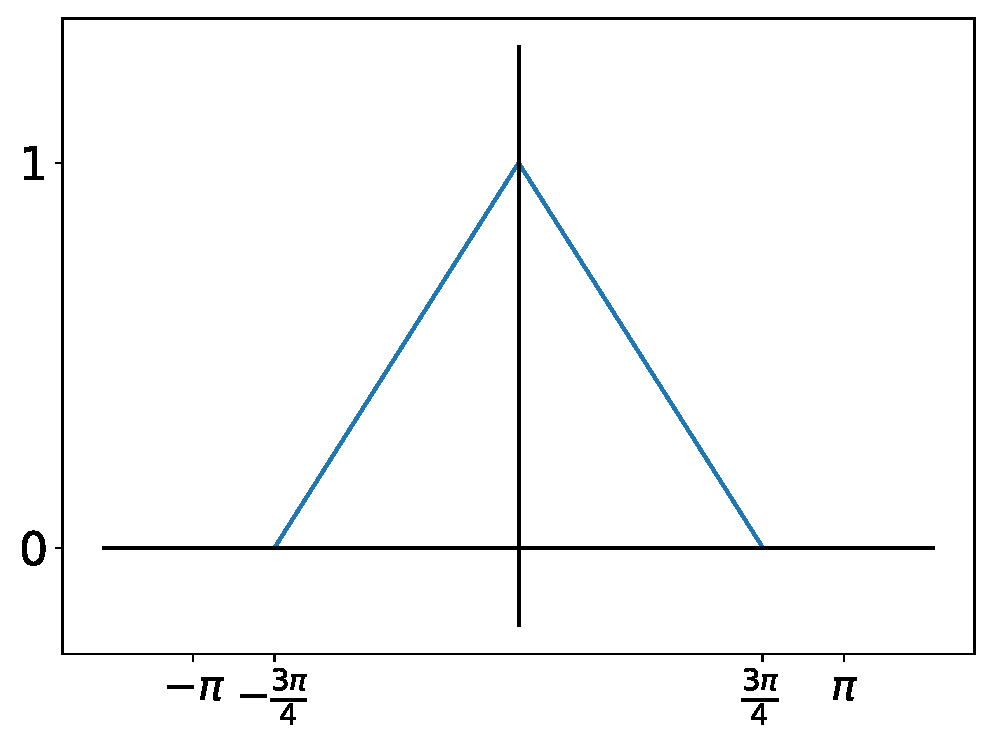
\includegraphics[width=63mm]{final_h2.eps}
\end{center}

پاسخ زمانی خروجی این سیستم را بیابید.

\end{document}